\section{Theorie}
\label{sec:Theorie}

Ziel dieses Versuches ist die Untersuchung des Relaxionsverhaltens eines RC-Kreises,
sowie demjenigen unter Anschluss von Gleich- oder Wechselstrom. \\

\subsection{Das Relaxionsverhalten}

Die Relaxion beschreibt die nicht-oszillatorische Rückkehr eines Systems in einen
Grundzustand, aus dem es zuvor gebracht wurde. Diese Rückkehr zum Endzustand $A(\infty)$
ist dabei nur asymptotisch möglich. Außerdem ist die Änderungsgeschwindigkeit proportional
zum Abstand der Größe $A$ zu ihrem Endzustand $A(\infty)$.

\begin{equation}
    \frac{\text{d}A}{\text{d}t} = c \left[A(t) - A(\infty) \right]
    \label{eqn:Aenderung}
\end{equation}

Durch Integration von \eqref{eqn:Aenderung} über $t$ von $\SI{0}{}$ bis $t$ ergibt
sich

\begin{equation}
    A(t) = A(\infty) + \left[A(0) - A(\infty) \right] \cdot \text{e}^{ct} \; \text{.}
    \label{eqn:Integration}
\end{equation}

Allerdings muss, damit A beschränkt ist, $c < 0$ in \eqref{eqn:Integration} gelten.
Im Folgenden soll das Relaxionsverhalten für das Beispiel eines über einen Widerstand
auf- und entladenden Kondensators nach Abbildung \ref{fig:sch_auf_ent} betrachtet werden.

\begin{figure}
\centering
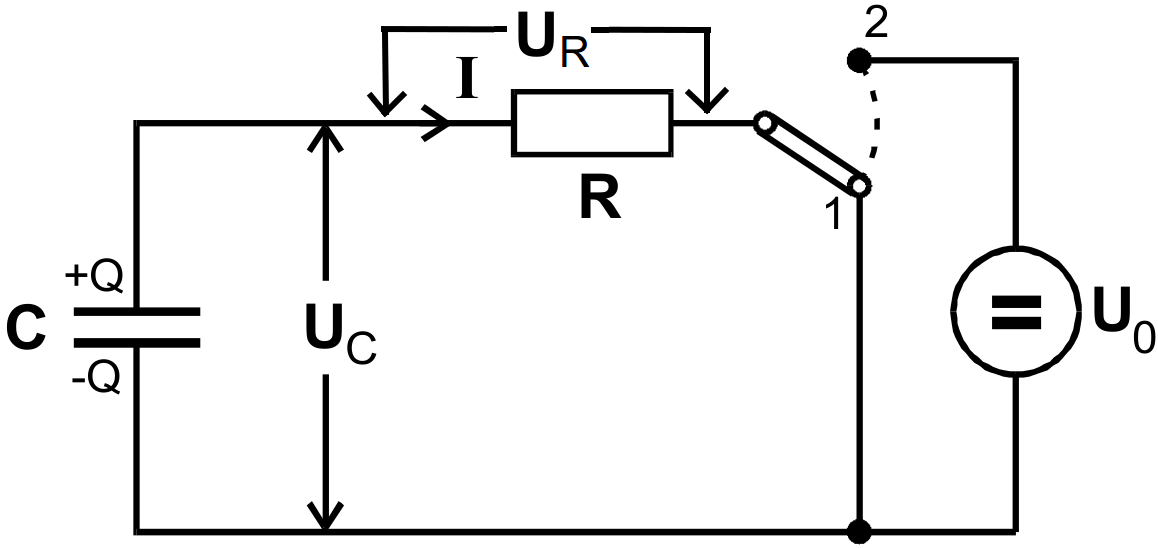
\includegraphics[scale=0.2]{content/Schaltung-auf-ent.png}
\caption{Aufladung (Stellung 2) und Entladung (Stellung 1) eines Kondensators über einen Widerstand [1]}
\label{fig:sch_auf_ent}
\end{figure}

\subsection{Die Auf- und Entladung eines Kondensators}

Liegt an dem Kondensator mit der Kapazität $C$ eine Ladung $Q$ vor, so liegt dort die Spannung 

\begin{equation*}
    U_\text{C} = \frac{Q}{C}
\end{equation*}

an. Mit dem Zusammenhang

\begin{equation*}
    I = - \frac{\text{d}Q}{\text{d}t} = \frac{U_\text{C}}{R}
\end{equation*}

ergibt sich für die Ladung $Q$ ähnlich zu \eqref{eqn:Aenderung}
 die zeitliche Differentialgleichung

\begin{equation}
    \dot{Q}(t) = - \frac{1}{RC} \cdot Q(t) \; \text{.}
\end{equation}

Mit der Randbedingung $Q(\infty) = 0$, dass der Kondensator sich nach einer unendlich langen Zeitspanne
vollständig entladen hat, ergibt sich nach \eqref{eqn:Integration} die Lösung

\begin{equation}
    Q(t) = Q(0) \cdot \text{e}^{\frac{-t}{RC}} \; \text{.}
    \label{eqn:ent}
\end{equation}

Analog führt der Aufladevorgang mit den Randbedingungen $Q(0) = 0 \text{  und  } Q(\infty) = CU_0$
zu der Lösung

\begin{equation}
    Q(t) = CU_0 \cdot \left(1 - \text{e}^{\frac{-t}{RC}}\right) \; \text{.}
\end{equation}

Der Ausdruck $RC$ wird als Zeitkonstante bezeichnet und gibt an, wie schnell das System seinem 
Endzustand entgegenstrebt.

\subsection{Die Relaxionsphänomene bei periodischer Auslenkung}

Als Beispiel für Relaxionsphänomene wird das Verhalten eines RC-Kreises bei anliegender
Sinusspannung nach Abbildung \ref{fig:sch_per} betrachtet. 

\begin{figure}
\centering
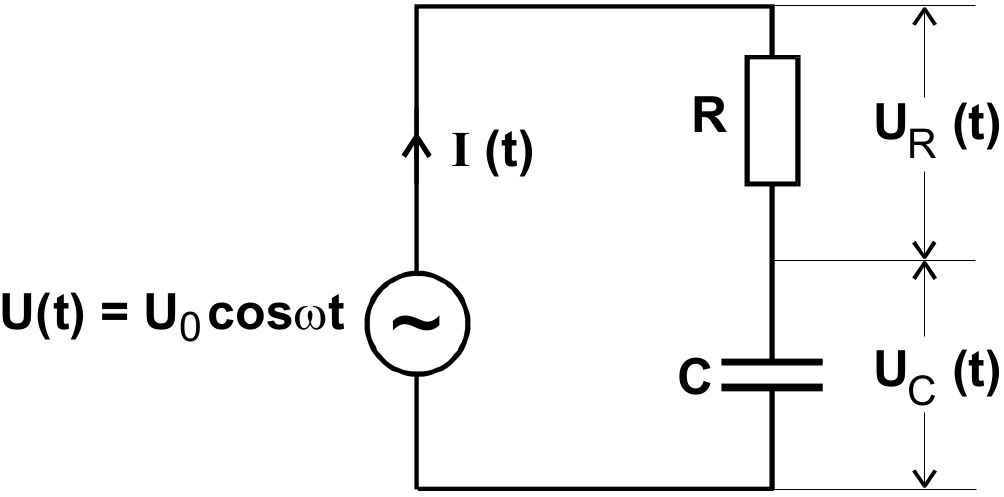
\includegraphics[scale=0.2]{content/sch_per.png}
\caption{Schaltung zur Untersuchung von Relaxationsphänomenen bei periodischer Auslenkung [1]}
\label{fig:sch_per}
\end{figure}

An der Schaltung liegt die Spannung

\begin{equation}
    U(t) = U_0 \cdot \text{cos}(\omega t)
\end{equation}

an. Ist die Kreisfrequenz $\omega << \frac{1}{RC}$ hinreichend klein, ist zu jedem Zeitpunkt
$U_\text{C} = U(t)$. Bei einer Erhöhung von $\omega$ tritt zwischen den Spannungen eine
Phasenverschiebung $\varphi$ auf und die Amplitude $A$ nimmt wegen des Zurückbleibens des
Auf- und Entladevorgangs des Kondensators hinter dem zeitlichen Verlauf von $U(t)$ ab. 

Mit einem Ansatz

\begin{equation*} 
    U_\text{C}(t) = A(\omega) \text{cos}(\omega t + \varphi(\omega))
\end{equation*}

ergibt sich unter Zuhilfenahme des 2. Kirchhoffschen Gesetzes und des Zusammenhangs

\begin{equation}
    \label{eqn:Stromstaerke}
    I(t) = \frac{\text{d}Q}{\text{d}t} = C \cdot \frac{\text{d}U_\text{C}}{\text{d}t}
\end{equation}

die Gleichung

\begin{equation}
    \label{eqn:Stromkreis}
    \begin{split}
        U(t) &= U_\text{R}(t) + U_\text{C}(t) \\
        U_0 \, \text{cos}(\omega t) &= -A(\omega) \, \omega RC \, \text{sin}(\omega t + \varphi)
        A(\omega) \, \text{cos}(\omega t + \varphi) 
    \end{split}
\end{equation}

Daraus folgen für die Phasenverschiebung $\varphi(\omega)$ und die Amplitude $A(\omega)$
die Gleichungen

\begin{equation}
    \varphi(\omega) = \text{arctan}(- \omega RC),
    \label{eqn:Phase}
\end{equation}

\begin{equation}
    A(\omega) = \frac{U_0}{\sqrt{1 + (\omega RC)^2}}.
    \label{eqn:Amplitude}
\end{equation}

Es ist zu erkennen, dass für niedrige Frequenzen die Phase $\varphi(\omega) \to 0$ und
die Amplitude $A(\omega) \to U_0$ gegen entsprechende Werte streben. Für größere
Frequenzen gilt hingegen $\varphi(\omega) \to \frac{\pi}{2}$ und $A(\omega) \to 0$.

\subsection{Der RC-Kreis als Integrator}

Unter den Bedingungen 

\begin{align*}
    \omega &>> \frac{1}{RC} \\
    \implies |U_\text{C}| &<< |U_\text{R}| \text{  und  } |U_\text{C}| << |U|
\end{align*}

kann der RC-Kreis die anliegende zeitlich veränderliche Spannung $U(t)$ integrieren.
Aus den Gleichungen \eqref{eqn:Stromkreis} und \eqref{eqn:Stromstaerke} ergibt sich die
Gleichung 

\begin{equation*}
    U(t) = RC \frac{\text{d}U_\text{C}}{\text{d}t} + U_\text{C}(t) \; \text{,}
\end{equation*}

die als

\begin{align*}
    U(t) &= RC \cdot \frac{\text{d}U_\text{C}}{\text{d}t} \\
    \iff U_\text{C}(t) &= \frac{1}{RC} \int^t_0 U(t') \; \text{d} t'
\end{align*}

genähert werden kann. Dabei ist $U_\text{C}(t)$ nur unter den oben genannten Bedingungen
proportional zu $\int U(t) \; \text{d}t$.

